\documentclass[conference,a4paper,10pt]{IEEEtran}
\IEEEoverridecommandlockouts

% ---- Paketler ----
\usepackage[T1]{fontenc}
\usepackage[utf8]{inputenc}
\usepackage{cite}
\usepackage{amsmath,amssymb}
\usepackage{graphicx}
\usepackage{xcolor}
\usepackage{listings}
\usepackage[ruled,vlined]{algorithm2e}
\usepackage{booktabs}
\usepackage{url}
\usepackage{hyperref}
\usepackage{multirow}

% ---- Türkçe etiketler ----
\renewcommand{\IEEEkeywordsname}{Anahtar Kelimeler}
\renewcommand{\figurename}{Şekil}
\renewcommand{\tablename}{Tablo}
\renewcommand{\refname}{Kaynaklar}

% ---- Kod renkleri ----
\definecolor{kodArka}{rgb}{0.97,0.97,0.97}
\definecolor{kodYorum}{rgb}{0.30,0.55,0.30}
\definecolor{kodAnahtar}{rgb}{0.10,0.30,0.70}
\definecolor{kodMetin}{rgb}{0.65,0.10,0.10}

% ---- Pseudo-code algoritma stili ----
\SetKwInput{KwGirdi}{Girdi}
\SetKwInput{KwCikti}{Cikti}
\SetKwFor{ForEach}{her}{icin yap}{son}

\begin{document}

\title{NoSQL'den SQL'e Dinamik Dönüşüm Sistemi:\\Şemasız JSON Verilerinin Otomatik\\İlişkisel Veritabanına Aktarımı}

\author{
\IEEEauthorblockN{Burak Kılcı \quad Ömer Faruk Teke}
\IEEEauthorblockA{
Bilgisayar Mühendisliği Bölümü\\
Kocaeli Üniversitesi\\
Kocaeli, Türkiye\\
230202111 \quad 210202045
}
}

\maketitle

% ====== ÖZET ======
\begin{abstract}
Bu çalışmada, yapısı önceden bilinmeyen JSON belgelerini çalışma zamanında analiz ederek otomatik olarak ilişkisel SQL veritabanına dönüştüren jenerik bir sistem geliştirilmiştir. Geliştirilen motor, iç içe geçmiş objeleri düzleştirme (\textit{flattening}) tekniğiyle tek tabloya indirgeyip dizileri Birinci Normal Form kuralı gereği ayrı alt tablolara ayırmakta ve ana tablo ile alt tablolar arasında otomatik Yabancı Anahtar bağlantıları kurmaktadır. Sistem ayrıca her sütun için en uygun SQL veri tipini (\texttt{INTEGER}, \texttt{REAL}, \texttt{TEXT}) tip çıkarımı yoluyla belirlemektedir. Python, Tkinter ve SQLite teknolojileriyle geliştirilen uygulama, dört farklı yapıdaki test JSON dosyasında, kodda tek bir satır değişiklik yapılmaksızın doğru tablo, ilişki ve veri tiplerini üretmiştir. Sistemin özyinelemeli yapısı, altı katmana kadar derinleşen iç içe yapıları başarıyla işleyebilmiş; bu durum, motorun farklı uygulama alanlarına uyarlanabilirliğini göstermiştir. Çalışmada elde edilen bulgular, NoSQL ve SQL paradigmaları arasında otonom bir köprü kurmanın mümkün olduğunu ve bu köprünün veri modelleme eğitiminde değerli bir araç olabileceğini ortaya koymaktadır.
\end{abstract}

\begin{IEEEkeywords}
NoSQL, SQL, JSON, dinamik şema, veri normalizasyonu, düzleştirme, ilişkisel veritabanı, Python, SQLite, otomatik dönüşüm
\end{IEEEkeywords}

% ====== I. GİRİŞ ======
\section{GİRİŞ}

Modern uygulamalarda JSON tabanlı NoSQL veri modelleri, esneklikleri ve şemasız yapıları nedeniyle yaygın biçimde tercih edilmektedir~\cite{nosql}. Web uygulamaları, mobil servisler, IoT cihazları ve REST tabanlı API'lar büyük çoğunlukla JSON formatını kullanmakta; veriyi insan tarafından okunabilir ve makinelerce kolay ayrıştırılabilir biçimde temsil etmektedir~\cite{json}. Ancak bu esneklik, raporlama, analitik sorgulama ve veri bütünlüğü açısından ilişkisel veritabanlarının sağladığı avantajları sınırlamaktadır~\cite{codd}. Karmaşık birleşim (\textit{join}) işlemleri, ACID özellikleri ve standartlaşmış bir sorgu dili olan SQL'in sunduğu olanaklar, ilişkisel modelin hâlâ güçlü olduğu noktalardır~\cite{date}.

Bu nedenle JSON verilerinin ilişkisel modele dönüştürülmesi, hibrit veri mimarilerinde sıkça karşılaşılan bir gereksinimdir. Geleneksel yaklaşımda, geliştirici hedef şemayı manuel olarak tasarlar ve dönüşüm kodunu \textit{hardcoded} biçimde yazar. Ancak bu yöntem, JSON şeması değiştiğinde kodun yeniden yazılmasını gerektirir ve büyük ölçekli, heterojen veri kaynaklarında pratik değildir.

Bu projenin amacı; yapısı, derinliği ve içerdiği alanlar önceden bilinmeyen herhangi bir JSON dosyasını okuyup, hiyerarşisini algoritmik olarak çözümleyen ve uygun ilişkisel tablolar ile ilişkileri (Birincil/Yabancı Anahtar) çalışma zamanında otomatik üreten jenerik bir dönüştürücü motoru tasarlamaktır. Tablo isimleri, sütun adları ve veri tipleri \textit{hardcoded} değil, tamamen girdi verisinden türetilmektedir. Bu sayede sistem, herhangi bir JSON yapısına önceden bilgi verilmeden uyarlanabilmektedir.

Geliştirilen sistem dört aşamadan oluşmaktadır: (i) JSON girdisinin okunup hiyerarşisinin analiz edilmesi, (ii) iç içe objelerin düzleştirilmesi ve ana tablo şemasının oluşturulması, (iii) dizilerin tespit edilerek alt tabloların ve Yabancı Anahtar ilişkilerinin kurulması, ve (iv) \texttt{CREATE TABLE} ve \texttt{INSERT INTO} sorgularının dinamik üretilip SQLite üzerinde yürütülmesi. Sistem ayrıca grafik bir kullanıcı arayüzüyle JSON ağacını ve sonuç tablolarını görsel olarak sunmaktadır.

Raporun geri kalanı şu şekilde düzenlenmiştir: Bölüm II ilgili çalışmaları ve mevcut yaklaşımları tartışmaktadır. Bölüm III sistemin mimarisini, akış diyagramını ve algoritmasını sunmaktadır. Bölüm IV örnek girdiler üzerinden üretilen şemaları, kullanım senaryolarını ve grafik arayüzü göstermektedir. Bölüm V elde edilen sonuçları, karmaşıklık analizini ve sınırlamaları değerlendirmektedir.

% ====== II. İLGİLİ ÇALIŞMALAR ======
\section{İLGİLİ ÇALIŞMALAR}

NoSQL ve SQL veritabanları arasında veri taşıma problemine yönelik literatürde çeşitli yaklaşımlar mevcuttur. \textbf{MongoDB BI Connector} gibi ticari araçlar, doküman tabanlı veriyi sanal ilişkisel görünümlere yansıtarak iş zekâsı uygulamalarının NoSQL kaynaklarına bağlanmasını sağlamaktadır. Ancak bu tür araçlar genellikle belirli bir veritabanı motoruna özgüdür ve genel amaçlı bir JSON-to-SQL dönüştürücü değildir.

JSON belgelerini ilişkisel modele yansıtan açık kaynaklı kütüphanelerden \textbf{json\_normalize} (Pandas) ve \textbf{flatten-json} gibi araçlar~\cite{pandas}, çoğunlukla yalnızca düzleştirme işlevini sunmakta; otomatik tablo bölünmesi ve Yabancı Anahtar yönetimi gibi normalizasyon adımlarını içermemektedir. Bu araçlar tüm JSON'u tek bir düz tabloya çevirir; iç içe diziler kayıp veriye veya satır çoğalmasına yol açar.

XML için tarihsel olarak geliştirilmiş \textbf{shredding} teknikleri~\cite{shredding}, hiyerarşik belgeleri ilişkisel tablolara bölmek için benzer prensipler kullanır. Ancak XML'in katı şeması, JSON'un şemasız doğasıyla doğrudan uyuşmaz; bu nedenle XML için geliştirilmiş yöntemler doğrudan uygulanamamaktadır.

Akademik literatürde, \textbf{schema discovery} (şema keşfi) konusunda yapılan çalışmalar, JSON koleksiyonlarından örtük şemaları çıkarmaya odaklanmaktadır~\cite{schemadisc}. Bu çalışmalar büyük ölçekli veri kümelerinde örnekleme ve tip çıkarımı yapan istatistiksel yöntemler önermektedir. Ancak bunlar genellikle pasif analiz araçlarıdır; üretilen şemayı doğrudan çalıştırılabilir SQL'e dönüştürmezler.

Bu çalışmanın özgün yanı; tek bir JSON belgesinin yapısından yola çıkarak tip çıkarımı, normalizasyon ve SQL üretimini bütünleşik biçimde gerçekleştiren \textit{kompakt}, \textit{eğitim odaklı} ve \textit{tamamen jenerik} bir motor sunmasıdır. Sistem, ticari araçların aksine herhangi bir bağımlılık veya lisans gerektirmeden tek bir Python kurulumuyla çalışmaktadır.

% ====== III. YÖNTEM ======
\section{YÖNTEM}

\subsection{Sistem Mimarisi}

Geliştirilen uygulama, sorumlulukları açıkça ayrılmış üç sınıf etrafında yapılandırılmıştır (Şekil~\ref{fig:class}):

\begin{itemize}
    \item \textbf{\texttt{Donusturucu}}: JSON verisinin algoritmik analizinden sorumlu motordur. Hiyerarşiyi tarayarak sanal tablo şemasını oluşturur. Tip çıkarımı ve normalizasyon kararları bu sınıfta verilir. Saf Python ile yazılmış olup harici hiçbir bağımlılığı yoktur.
    \item \textbf{\texttt{VeritabaniYazici}}: Üretilen sanal şemayı gerçek SQLite veritabanına yansıtan modüldür. \texttt{CREATE TABLE} ve \texttt{INSERT INTO} sorgularını parametreli biçimde üretir ve topolojik sırayla yürütür; böylece Yabancı Anahtar kısıtlamaları her zaman geçerli kalır.
    \item \textbf{\texttt{Uygulama}}: Tkinter tabanlı grafik arayüzdür. Kullanıcı eylemlerini koordine eder, JSON ağacını ağaç görünümünde, oluşan tabloları ise sekmeli DataGrid biçiminde görselleştirir.
\end{itemize}

\begin{figure}[!ht]
\centering
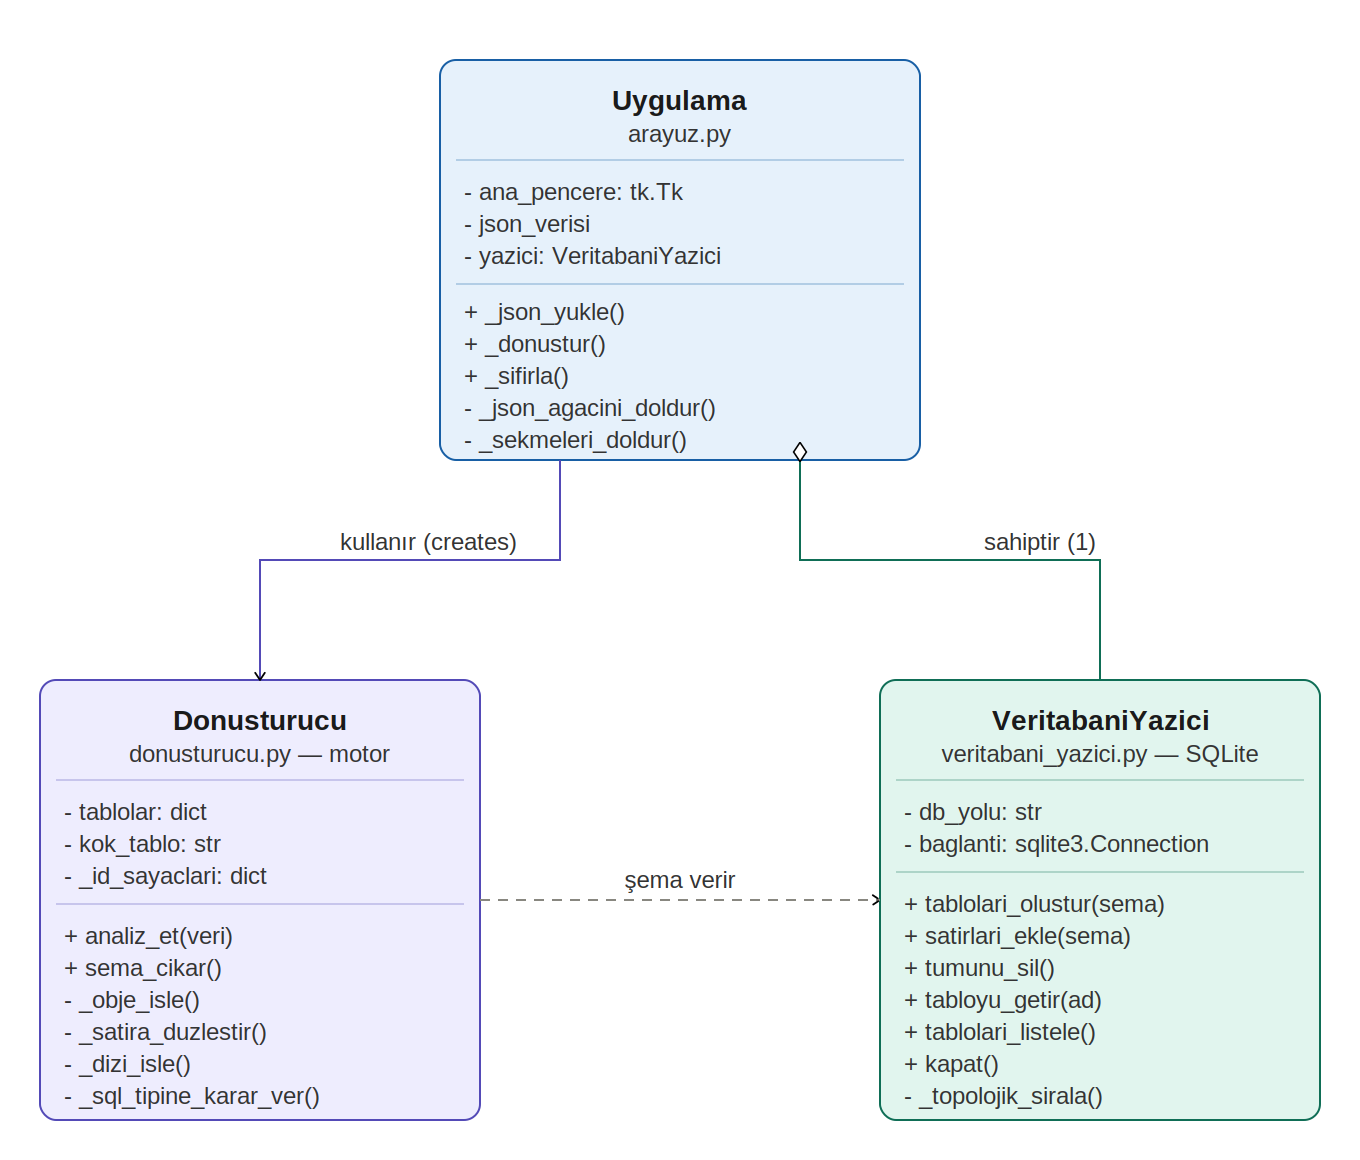
\includegraphics[width=\columnwidth]{figures/class_diagram.png}
\caption{Sistemin sınıf diyagramı. \texttt{Uygulama} arayüz katmanı; \texttt{Donusturucu} ve \texttt{VeritabaniYazici} ile sırasıyla \textit{kullanır} ve \textit{sahiptir} ilişkilerinde bulunur.}
\label{fig:class}
\end{figure}

Modüller arasındaki iletişim sade ve tek yönlüdür: \texttt{Uygulama} kullanıcıdan gelen olaylara karşılık önce \texttt{Donusturucu}'yu çağırarak sanal şema sözlüğünü elde eder, ardından bu sözlüğü \texttt{VeritabaniYazici}'ye geçirerek fiziksel tabloların oluşturulmasını sağlar. Bu mimari, motorun arayüzden bağımsız test edilebilmesine de olanak tanımaktadır.

\subsection{Sistem Akış Diyagramı}

Sistemin uçtan uca işleyişi Şekil~\ref{fig:akis}'te akış diyagramı olarak gösterilmiştir. Akış, JSON dosyasının yüklenmesinden başlayarak son olarak oluşturulan tabloların kullanıcıya sunulmasıyla tamamlanmaktadır. Her bir düğüm tipi (primitif, obje, dizi) için farklı bir kontrol akışı izlenmektedir.

\begin{figure}[!ht]
\centering
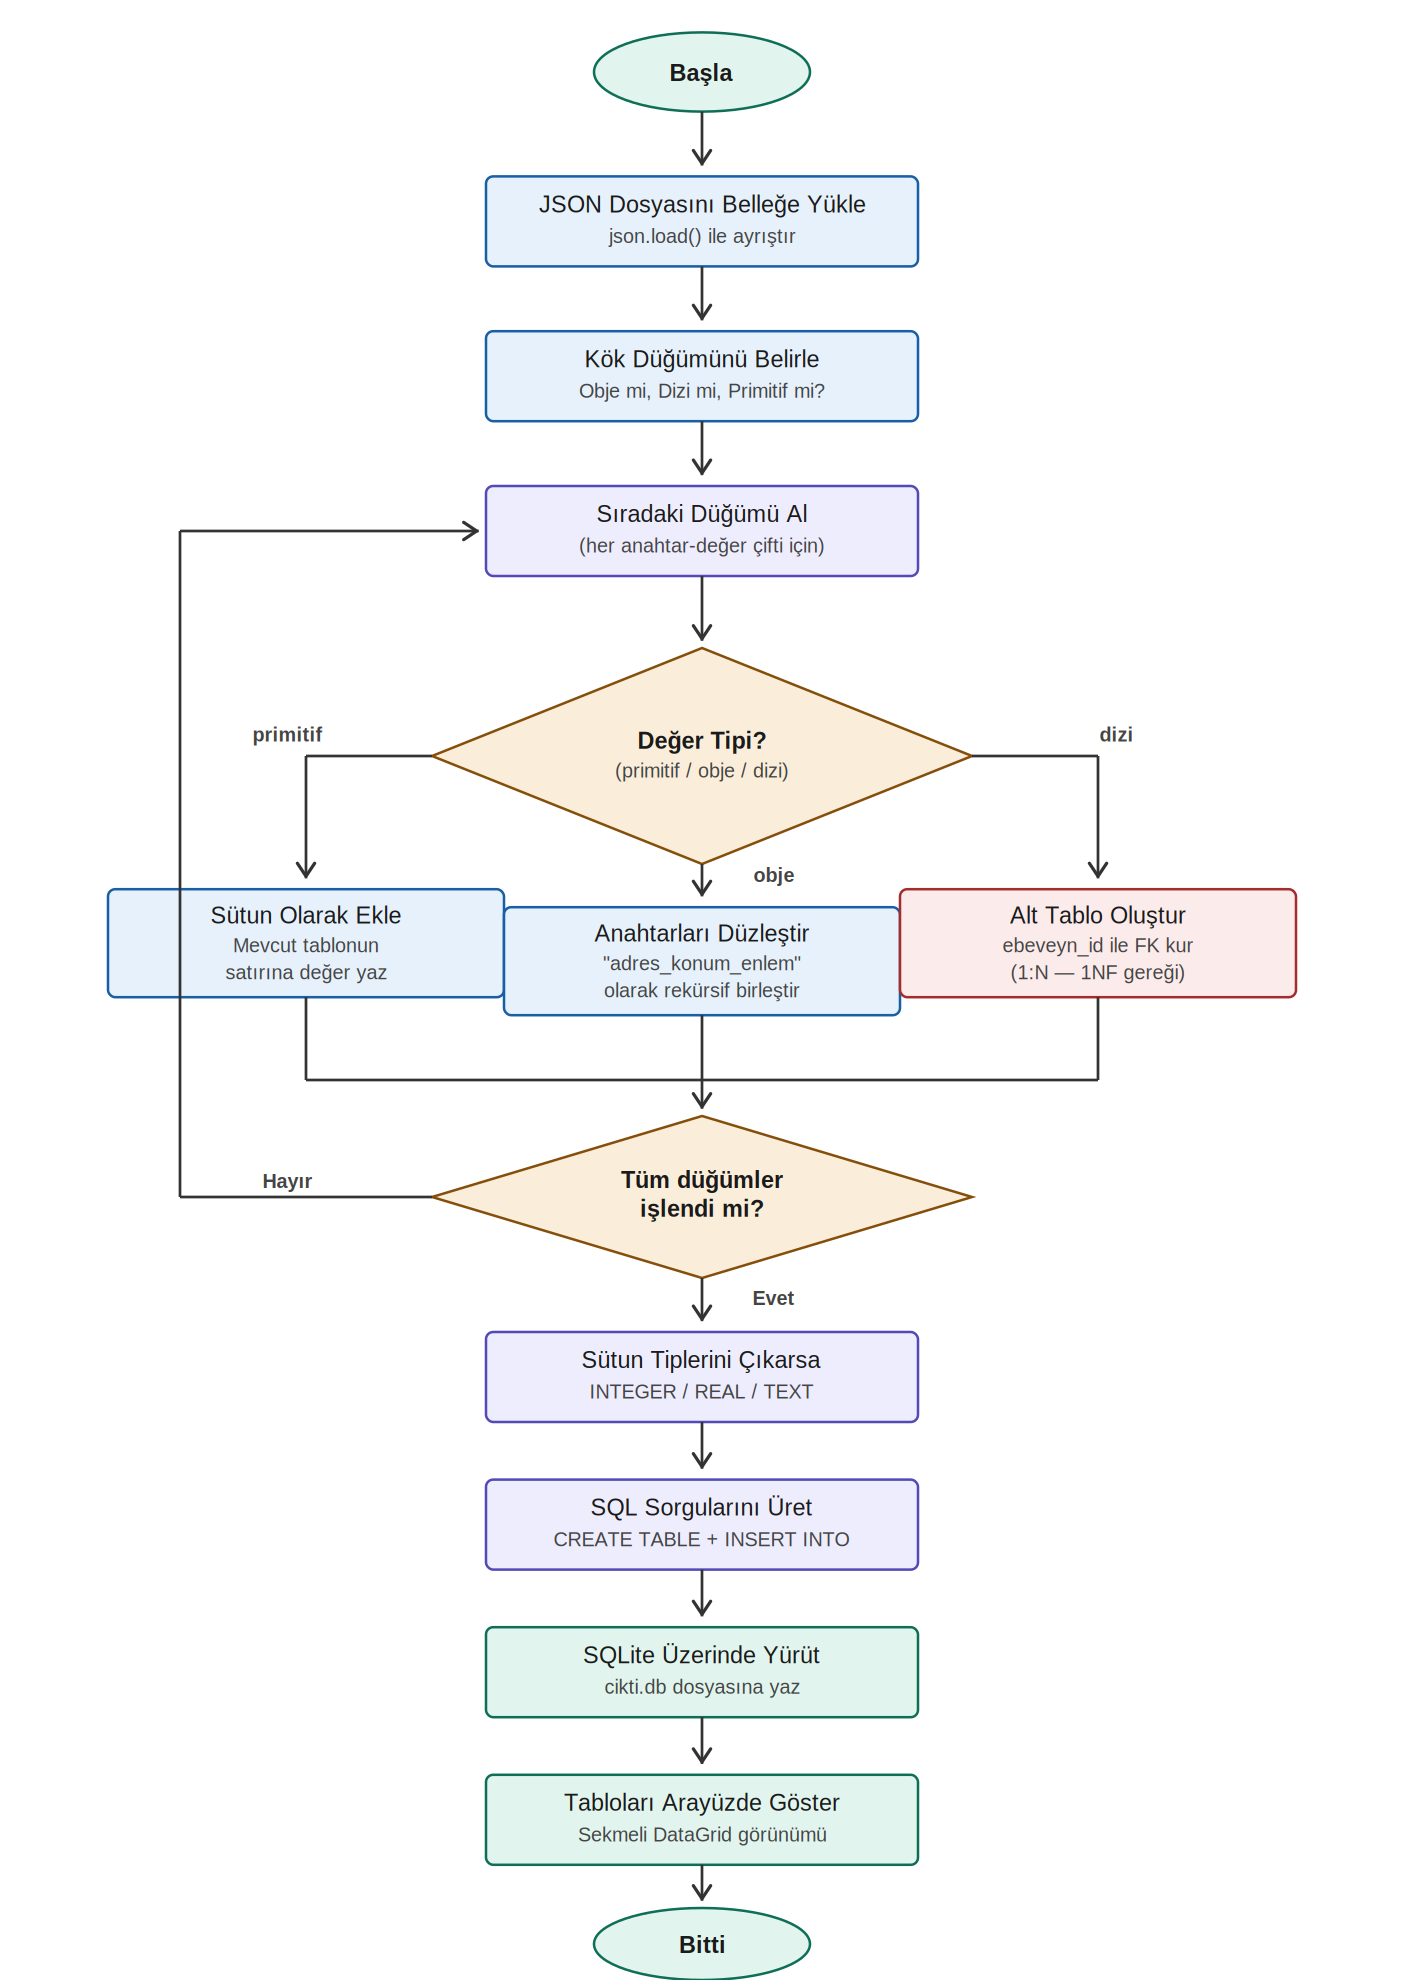
\includegraphics[width=0.95\columnwidth]{figures/akis_diyagrami.png}
\caption{Sistemin yüksek seviyeli akış diyagramı. Karar düğümleri, JSON içindeki her elemanın tipini analiz ederek uygun işleme yönlendirir.}
\label{fig:akis}
\end{figure}

\subsection{Düzleştirme (Flattening) Stratejisi}

Algoritma, iç içe geçmiş objelerle karşılaştığında bunları ana tablo içinde tek bir satır düzlemine indirgemektedir. Örneğin \texttt{adres.konum.enlem} ifadesi, ebeveyn ve çocuk anahtarları alt çizgi karakteriyle birleştirilerek \texttt{adres\_konum\_enlem} biçiminde tek bir sütuna dönüştürülür. Bu işlem rekürsif yapılır ve teorik olarak sınırsız derinlikteki objeleri destekler. Pratikte ise kullanıcı arayüzü ve okunabilirlik açısından 5-6 katmana kadar derinleşen yapılar test edilmiş ve başarıyla işlenmiştir.

Düzleştirme stratejisinin tercih edilme sebebi, iç içe objelerin genellikle ana varlığa ait \textit{tek değerli} (1:1) öznitelikler olmasıdır. Örneğin bir kullanıcının adresi ve adresinin koordinatları, ayrı tablolara bölünmek yerine ana kullanıcı kaydında saklanırsa hem JOIN maliyetinden kaçınılmış hem de okuma performansı artırılmış olur.

\subsection{Dizi Yönetimi ve Normalizasyon}

İlişkisel modelde aynı satırda birden fazla atomik olmayan değerin saklanması Birinci Normal Form'u (1NF) ihlal eder~\cite{codd}. Bu durum, sorguların karmaşıklaşmasına ve veri tutarsızlıklarına yol açar~\cite{date}. Bu nedenle algoritma bir dizi (\texttt{[\dots]}) yapısı tespit ettiğinde aşağıdaki adımları izlemektedir:

\begin{enumerate}
    \item Yeni bir alt tablo \texttt{ebeveyn\_dizianahtar} adıyla otomatik oluşturulur.
    \item Alt tabloya \texttt{id} (Birincil Anahtar) ve \texttt{ebeveyn\_id} (Yabancı Anahtar) sütunları eklenir.
    \item Dizinin her elemanı alt tabloda ayrı bir satır olarak yazılır.
    \item Eleman bir obje ise düzleştirme rekürsif olarak uygulanır; primitif ise tek sütunda (\texttt{deger}) saklanır.
    \item İç içe diziler için süreç özyinelemeli olarak devam eder; bu sayede 5--6 katman derinlikteki yapılar Üçüncü Normal Form'a uygun olarak ayrı tablolara bölünür.
\end{enumerate}

Tablo~\ref{tab:nf}, geliştirilen sistemin sağladığı normalizasyon kurallarını ve her birinin nasıl uygulandığını özetlemektedir.

\begin{table}[!ht]
\caption{Sistemin Sağladığı Normalizasyon Kuralları}
\label{tab:nf}
\centering
\footnotesize
\renewcommand{\arraystretch}{1.3}
\begin{tabular}{@{}p{1.4cm}p{2cm}p{3.5cm}@{}}
\toprule
\textbf{Form} & \textbf{Kural} & \textbf{Uygulama} \\
\midrule
1NF & Atomik değerler & Diziler ayrı alt tabloya ayrılır \\
2NF & Birincil anahtar & Her tabloya otomatik \texttt{id} sütunu eklenir \\
3NF & Geçişli bağımlılık yok & İç içe yapılar ayrı tablolara bölünür, FK ile bağlanır \\
\bottomrule
\end{tabular}
\end{table}

\subsection{Tip Çıkarımı}

Sütun veri tipleri, ilgili sütunda gözlemlenen tüm Python tiplerinin birleşim kümesinden çıkarsanır. Çıkarım işleminde \texttt{None} değerleri göz ardı edilerek tipte iyimser kalınır; karışım durumunda ise her zaman bilgi kaybetmeyen üst tip seçilir. Tablo~\ref{tab:tip} olası Python tipi kümeleri ile bu tiplere karşılık gelen SQL tiplerini özetlemektedir.

\begin{table}[!ht]
\caption{Python Tipi Kümesinden SQL Tipine Eşleme}
\label{tab:tip}
\centering
\footnotesize
\renewcommand{\arraystretch}{1.2}
\begin{tabular}{@{}lcc@{}}
\toprule
\textbf{Gözlenen Python tipleri} & \textbf{SQL tipi} & \textbf{Örnek alan} \\
\midrule
\{int\}                       & INTEGER & yas, kontenjan \\
\{int, bool\}                 & INTEGER & sayilar + bayraklar \\
\{int, float\}                & REAL    & puan, fiyat \\
\{bool\}                      & INTEGER & aktif, secmeli \\
\{str\}                       & TEXT    & ad, sehir \\
\{str, int\} (karışık)        & TEXT    & değişken alan \\
\{null\} (yalnızca)           & TEXT    & varsayılan \\
\bottomrule
\end{tabular}
\end{table}

Tip çıkarımı kuralı, motor içinde aşağıdaki gibi tek bir saf fonksiyonla ifade edilmiştir:

\begin{verbatim}
def sql_tipine_karar_ver(python_tipleri):
    null_olmayan = python_tipleri - {"null"}
    if not null_olmayan:
        return "TEXT"
    if null_olmayan == {"bool"}:
        return "INTEGER"
    if null_olmayan <= {"int", "bool"}:
        return "INTEGER"
    if null_olmayan <= {"int","float","bool"}:
        return "REAL"
    return "TEXT"
\end{verbatim}

\subsection{Algoritmanın Yalancı Kodu}

Sistemin merkezindeki obje ve dizi işleme rutinleri sırasıyla Algoritma~\ref{alg:obje_isle} ve Algoritma~\ref{alg:dizi_isle} ile özetlenmiştir. Bu iki rutin birbirini özyinelemeli olarak çağırarak JSON'un tüm hiyerarşisini gezmektedir.

\begin{algorithm}
\DontPrintSemicolon
\caption{Obje İşleme ve Şema Üretimi}
\label{alg:obje_isle}
\KwGirdi{$obje$, $tabloAdi$, $ebeveynId$, $ebeveynTablo$}
\KwCikti{Bu objeye atanan satır kimliği $satirId$}
\BlankLine
$tabloyuHazirla(tabloAdi, ebeveynTablo)$\;
$satirId \leftarrow sonrakiId(tabloAdi)$\;
$duzSatir \leftarrow \{\,id : satirId\,\}$\;
\If{$ebeveynId \neq null$}{
  $duzSatir.ebeveynId \leftarrow ebeveynId$\;
}
$diziler \leftarrow \emptyset$\;
\ForEach{$(anahtar, deger) \in obje$}{
  \If{$deger$ bir obje ise}{
    rekürsif olarak iç alanları \texttt{anahtar\_alt} adıyla $duzSatir$'a ekle\;
  }
  \ElseIf{$deger$ bir dizi ise}{
    $diziler \leftarrow diziler \cup \{(anahtar, deger)\}$\;
  }
  \Else{
    $duzSatir.anahtar \leftarrow deger$\;
  }
}
$duzSatir$'ı $tabloAdi$'ye satır olarak ekle\;
\ForEach{$(dAnahtar, dDeger) \in diziler$}{
  $altTablo \leftarrow tabloAdi + \texttt{"\_"} + dAnahtar$\;
  $diziIsle(dDeger, altTablo, satirId, tabloAdi)$\;
}
\Return $satirId$\;
\end{algorithm}

\begin{algorithm}
\DontPrintSemicolon
\caption{Dizi İşleme ve Alt Tablo Üretimi}
\label{alg:dizi_isle}
\KwGirdi{$dizi$, $tabloAdi$, $ebeveynId$, $ebeveynTablo$}
\BlankLine
\If{$dizi$ boş}{
  \KwRet{} \tcp*{Gereksiz iskelet tablo oluşturma}
}
$tabloyuHazirla(tabloAdi, ebeveynTablo)$\;
\ForEach{$eleman \in dizi$}{
  \uIf{$eleman$ bir obje ise}{
    $objeIsle(eleman, tabloAdi, ebeveynId, ebeveynTablo)$\;
  }
  \uElseIf{$eleman$ bir dizi ise}{
    $derinTablo \leftarrow tabloAdi + \texttt{"\_oge"}$\;
    Yeni satır oluştur, $diziIsle(eleman, derinTablo, satirId, tabloAdi)$\;
  }
  \Else{
    $deger$ alanına $eleman$ atanmış yeni satır ekle\;
  }
}
\end{algorithm}

\subsection{Dinamik SQL Üretimi}

JSON'un tüm hiyerarşisi tarandıktan sonra elde edilen sanal şema, parametreli SQL sorgularına dönüştürülür. Aşağıda \texttt{test\_data.json} girdisi için motor tarafından üretilen \texttt{CREATE TABLE} ifadelerinden bir kesit verilmiştir:

\begin{verbatim}
CREATE TABLE "test_data" (
  "id"          INTEGER PRIMARY KEY,
  "ad"          TEXT,
  "soyad"       TEXT,
  "yas"         INTEGER,
  "aktif"       INTEGER,
  "puan"        REAL,
  "adres_sehir" TEXT,
  "adres_ilce"  TEXT
);
CREATE TABLE "test_data_telefonlar" (
  "id"         INTEGER PRIMARY KEY,
  "ebeveyn_id" INTEGER REFERENCES test_data(id),
  "deger"      TEXT
);
\end{verbatim}

Yukarıdaki sorgular motor tarafından çalışma zamanında, JSON'daki anahtar adlarından ve değer tiplerinden türetilmiştir. Hiçbir tablo veya sütun adı kodda \textit{hardcoded} olarak yer almamaktadır. \texttt{INSERT INTO} sorguları ise SQL injection saldırılarına karşı parametreli (\texttt{?} yer tutucularıyla) yürütülmektedir.

\subsection{Kullanım Senaryoları}

Kullanıcının sistemle etkileşimi Şekil~\ref{fig:usecase}'de UML kullanım senaryosu diyagramı ile gösterilmiştir. Birincil aktör Kullanıcı; ikincil aktörler ise JSON dosyasını sağlayan Dosya Sistemi ve verileri saklayan SQLite Veritabanıdır. \texttt{«include»} ilişkileri, bir senaryonun zorunlu alt adımlarını; \texttt{«extend»} ise hata gibi koşullu durumlarda devreye giren ek senaryoları temsil etmektedir~\cite{uml}.

\begin{figure}[!ht]
\centering
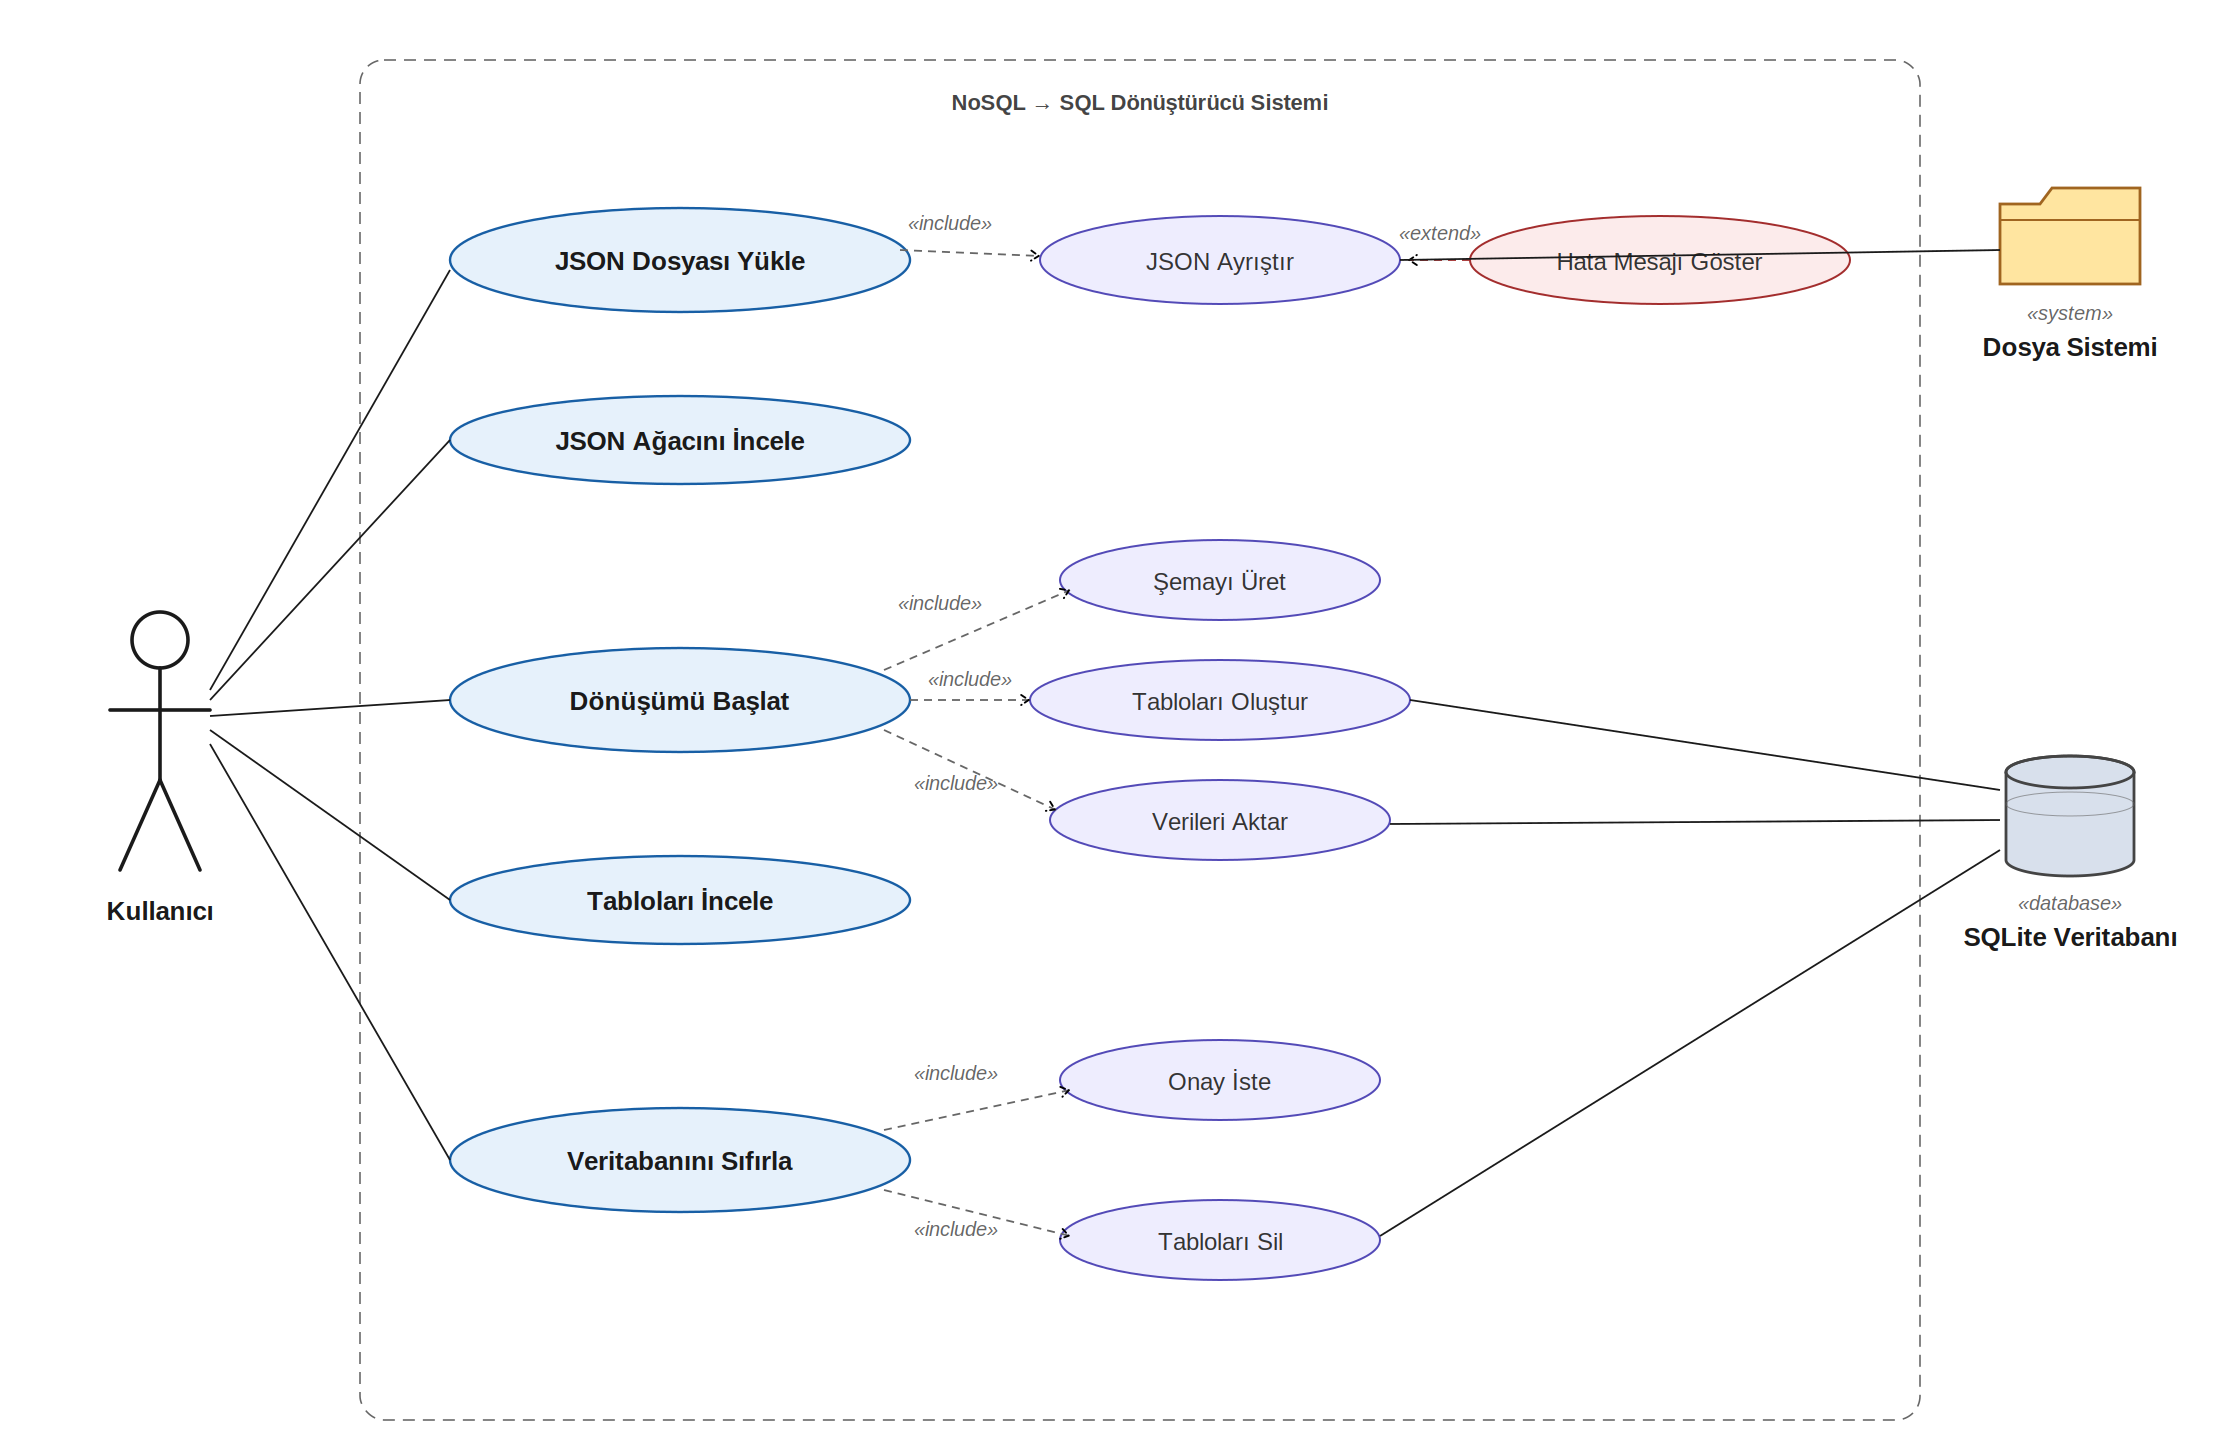
\includegraphics[width=\columnwidth]{figures/use_case_diagram.png}
\caption{Sistemin kullanım senaryosu (use case) diyagramı. Birincil aktör (Kullanıcı) ve ikincil aktörler (Dosya Sistemi, SQLite) sistemle olan etkileşim noktalarıyla birlikte gösterilmiştir.}
\label{fig:usecase}
\end{figure}

% ====== IV. ÖRNEK GÖRSELLER ======
\section{ÖRNEK GÖRSELLER VE UYGULAMA}

\subsection{Dinamik Olarak Üretilen Veritabanı Şeması}

Şekil~\ref{fig:er}, basit bir test JSON dosyasından (kullanıcı bilgileri, telefonlar, siparişler ve eğitim geçmişi) sistem tarafından otomatik üretilen veritabanı şemasını göstermektedir. Görüldüğü üzere ana tablonun yanı sıra dört alt tablo oluşturulmuş, her alt tabloya \texttt{ebeveyn\_id} alanı Yabancı Anahtar olarak yerleştirilmiştir. \texttt{egitim\_dersler} tablosu ise iki katmanlı hiyerarşinin sonucu olarak oluşmuş ve \texttt{egitim} tablosuna bağlanmıştır.

\begin{figure}[!ht]
\centering
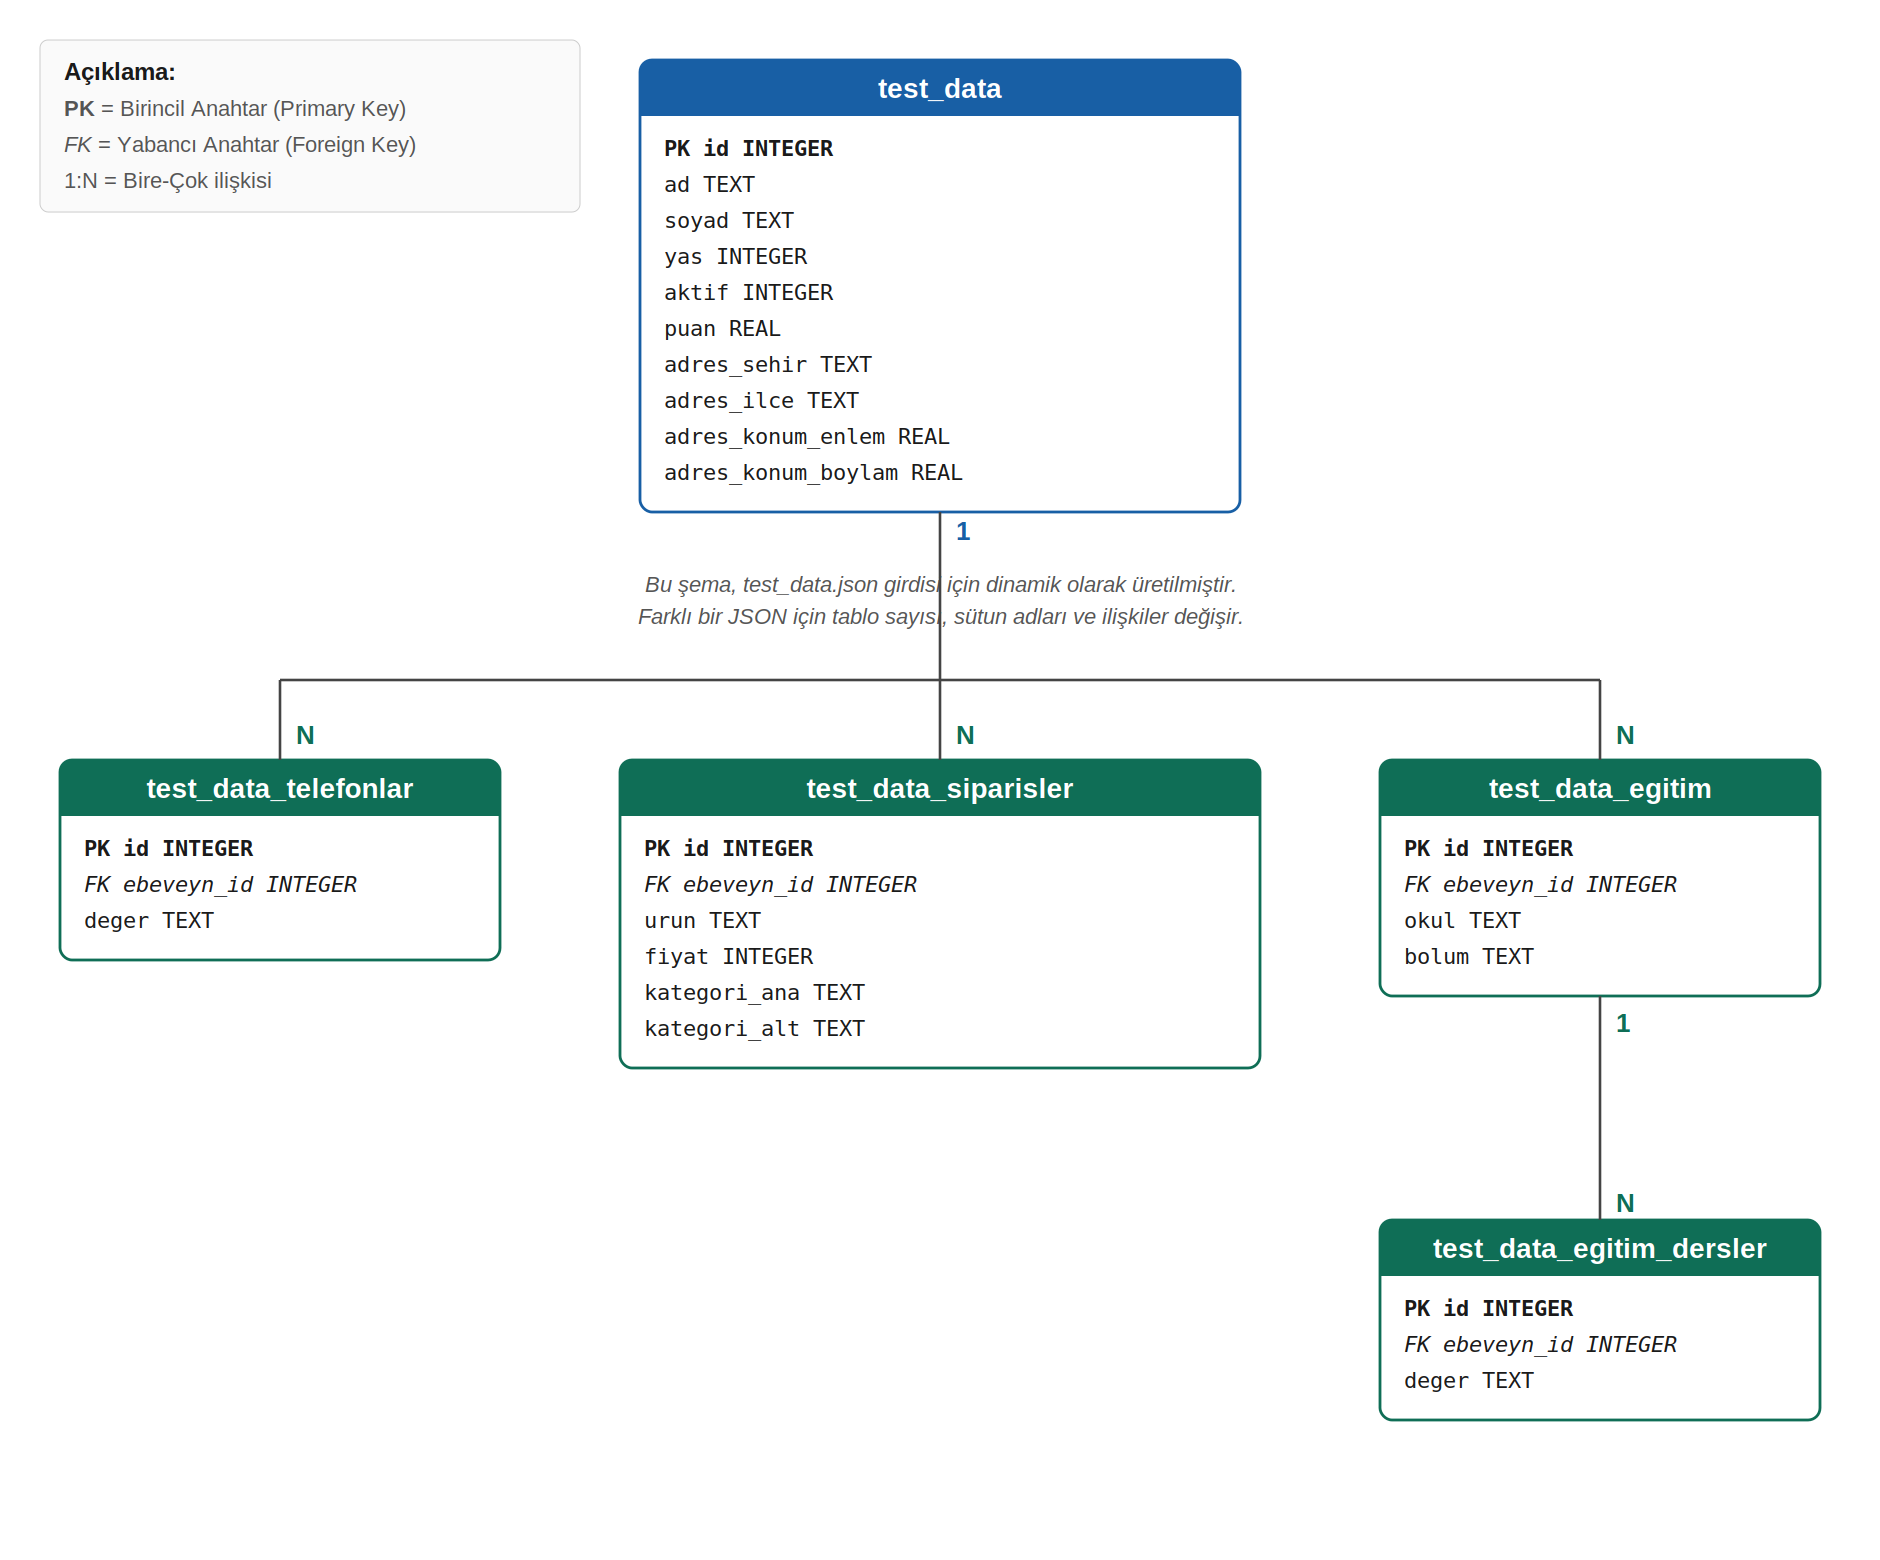
\includegraphics[width=\columnwidth]{figures/er_diagram.png}
\caption{\texttt{test\_data.json} girdisinden dinamik üretilmiş veritabanı şeması. Tablo sayısı, sütun adları ve ilişkiler farklı bir JSON için tamamen değişmektedir.}
\label{fig:er}
\end{figure}

Ana tablodaki \texttt{adres\_sehir}, \texttt{adres\_ilce}, \texttt{adres\_konum\_enlem} ve \texttt{adres\_konum\_boylam} sütunları, JSON'daki iki katmanlı \texttt{adres.konum} yuvalanmasının düzleştirme sonucudur. Bu örnek, hem düzleştirme hem de alt tablo üretimi mantığının aynı belge içinde nasıl birlikte çalıştığını göstermektedir.

\subsection{Grafik Kullanıcı Arayüzü}

Şekil~\ref{fig:gui}, geliştirilen Tkinter tabanlı arayüzü göstermektedir~\cite{tkinter}. Sol panel JSON hiyerarşisini ağaç görünümünde sunarken, sağ panel dönüşüm sonucu oluşan SQL tablolarını sekmeli yapıda DataGrid biçiminde göstermektedir. Alt durum çubuğu üretilen tablo ve satır sayısını anlık olarak raporlamaktadır. Üstteki üç buton (\textit{JSON Yükle}, \textit{Dönüştür}, \textit{Sıfırla}) sistemin temel kullanım senaryolarını tetiklemektedir.

\begin{figure}[!ht]
\centering
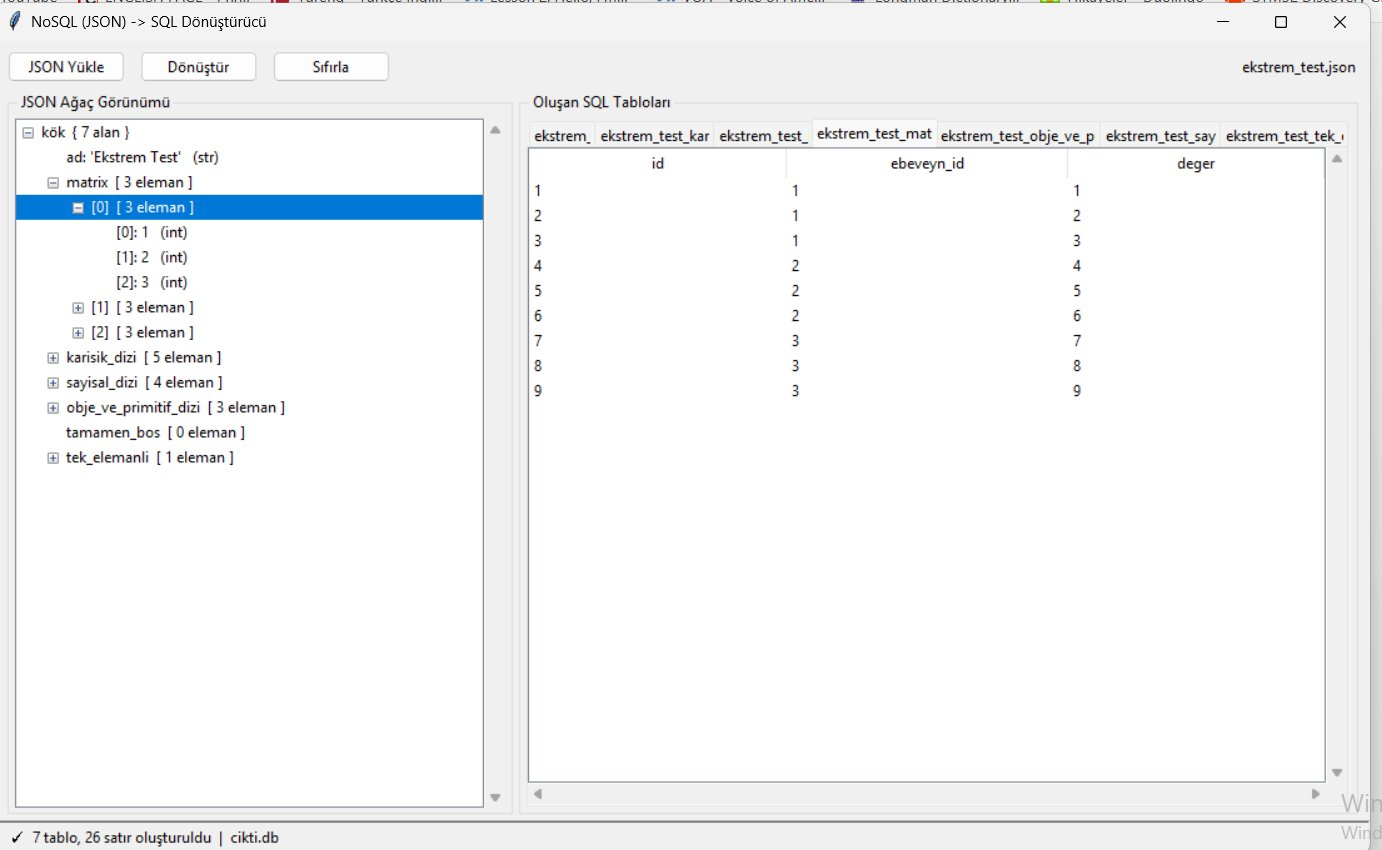
\includegraphics[width=\columnwidth]{figures/gui_screenshot.png}
\caption{Uygulamanın grafik arayüzü. Solda yüklenen JSON'un ağaç görünümü, sağda dönüşüm sonucu oluşan SQL tabloları sekmeli görünümle sunulmuştur.}
\label{fig:gui}
\end{figure}

JSON ağaç görünümünde her düğümün yanında parantez içinde değerin tipi (\texttt{int}, \texttt{str}, \texttt{bool} vb.) gösterilmektedir; bu kullanıcıya, motor tarafından yapılacak tip çıkarımının önizlemesini sunar. Sağ paneldeki sekmeli yapıda ise her tablo için ayrı bir sekme bulunur ve sekmeler arası geçiş yaparak farklı ilişkili tabloların içeriği rahatlıkla incelenebilir.

\subsection{Test Senaryoları}

Sistem, farklı yapısal özelliklere sahip dört JSON dosyası ile test edilmiş ve sonuçlar Tablo~\ref{tab:test} ile özetlenmiştir.

\begin{table}[!ht]
\caption{Test JSON Dosyaları ve Üretilen Şema İstatistikleri}
\label{tab:test}
\centering
\footnotesize
\begin{tabular}{@{}lccl@{}}
\toprule
\textbf{Test Dosyası} & \textbf{Tablo} & \textbf{Satır} & \textbf{Test Edilen Özellik} \\
\midrule
\texttt{test\_data.json}    & 5 & 9  & Temel düzleştirme, dizi \\
\texttt{zorlu\_test.json}   & 7 & 16 & 6 katman derinlik, null\\
\texttt{kok\_dizi\_test.json} & 2 & 6 & Kök dizi, eksik alanlar \\
\texttt{ekstrem\_test.json} & 7 & 26 & Matris, karışık tip\\
\bottomrule
\end{tabular}
\end{table}

\textbf{\texttt{zorlu\_test.json}} senaryosu özellikle önemli bir test olmuştur. Bu dosya, bir üniversite yapısını altı katman derinlikte modellemektedir: \emph{üniversite -- fakülteler -- bölümler -- dersler -- öğrenciler -- notlar}. Sistem bu yapı için yedi farklı tablo üretmiş, en derin tablonun (\texttt{notlar}) ana tabloya kadar doğru zincirleme Yabancı Anahtar bağlantılarını kurmuştur.

\textbf{\texttt{ekstrem\_test.json}} ise kenar durumları test etmek üzere tasarlanmış olup matris (iç içe sayı dizileri), karışık tipli diziler (metin + sayı + boolean), boş diziler ve tek elemanlı diziler içermektedir. Sistem bu dosya için yirmi altı satır üretmiş ve hiçbir hata vermeden işlemini tamamlamıştır.

% ====== V. SONUÇ ======
\section{SONUÇ}

Bu çalışmada, şemasız JSON verilerini otomatik olarak ilişkisel SQL veritabanına aktaran jenerik bir dönüştürücü motor başarıyla geliştirilmiştir. Sistem; iç içe objelerin düzleştirilmesi, dizilerin alt tablolara ayrılması, otomatik Birincil ve Yabancı Anahtar yönetimi ile veri tipi çıkarımı işlevlerini bütünleşik biçimde sunmaktadır.

Önemli bir başarı kriteri, geliştirilen kodun herhangi bir test senaryosuna bağımlı (\textit{hardcoded}) olmamasıdır. Birbirinden farklı yapıdaki dört test dosyası, kodda hiçbir değişiklik yapılmaksızın doğru biçimde dönüştürülmüştür. Üretilen veritabanı şemaları 1NF, 2NF ve 3NF normalizasyon kurallarını sağlamaktadır~\cite{normalformler}.

Geliştirme sürecinde edinilen tecrübe, NoSQL ve SQL paradigmaları arasındaki temel farkın yalnızca sözdizimsel değil, semantik olduğunu da göstermiştir. Şemasız JSON modeli, aynı kavramı (``ad-soyad'', ``adres-konum'') farklı derinliklerde ve farklı isimlendirmelerle ifade edebildiği için, dönüşümde yapay isim çakışmalarının (\textit{name collision}) önlenmesi ve hiyerarşinin tutarlı biçimde Yabancı Anahtarlarla temsili kritik teknik kararlar olarak ortaya çıkmıştır. Sistemin özyinelemeli yapısı, ileride çok daha derin ve heterojen JSON kaynaklarına da uyarlanmasına olanak tanımaktadır.

\subsection{Karmaşıklık Analizi}

Algoritmanın çalışma süresi, JSON belgesindeki toplam düğüm sayısı $n$ ile doğrusal orantılıdır. Her düğüm yalnızca bir kez ziyaret edildiğinden zaman karmaşıklığı $\mathcal{O}(n)$'dir. Düzleştirme işleminde rekürsif derinlik, JSON'un en derin obje yuvalanmasıyla sınırlıdır; pratikte bu derinlik 10'u nadiren geçtiğinden bellek tüketimi sabit sayılabilir. \texttt{INSERT} işlemleri SQLite'in transaksiyon yönetimi sayesinde tek toplu işlemde gerçekleşmekte, bu da disk yazma maliyetini önemli ölçüde azaltmaktadır~\cite{sqlite}.

Tablo sayısı $t$ olduğunda, \texttt{CREATE TABLE} sorgularının topolojik sıralaması $\mathcal{O}(t)$ zamanında gerçekleştirilmektedir. Toplamda algoritmanın asimptotik karmaşıklığı $\mathcal{O}(n + t)$ olup pratikte $t \ll n$ olduğundan, sistem büyük JSON dosyalarında dahi doğrusal performans göstermektedir.

\subsection{Sınırlamalar ve Tartışma}

Geliştirilen sistemin mevcut sürümünde bazı sınırlamalar bulunmaktadır. Birincisi, tüm JSON belgesi belleğe yüklenmektedir; bu, gigabayt mertebesindeki dosyalar için bellek darboğazına yol açabilir. Bu sorun, akış (\textit{streaming}) tabanlı JSON ayrıştırıcılarla aşılabilir.

İkincisi, alt tablo isimleri ebeveyn-anahtar birleşimiyle üretildiğinden çok derin yapılarda tablo adları uzayabilir. Örneğin altı katman derinlikteki bir yapı için tablo adı 60 karakteri aşabilir; bazı veritabanı motorlarında bu sınırı zorlayabilir. Çözüm olarak, anlamlı kısaltma stratejileri veya hash tabanlı isim üretimi uygulanabilir.

Üçüncüsü, motor şu an SQLite'a özel bazı tip eşleşmelerine güvenmektedir; PostgreSQL veya MySQL'e taşıma için \texttt{BOOLEAN} ve \texttt{NUMERIC} gibi ek tiplerin desteklenmesi gerekmektedir. Veritabanı motoruna özgü dialekt yöneticisi eklenerek bu durum çözülebilir.

Bu sınırlamalar, projenin akademik kapsamı içinde değil ama endüstriyel kullanım senaryoları için anlamlıdır. Yine de mevcut motor, NoSQL-SQL köprüleme görevini başarıyla yerine getirmekte ve ilişkisel veritabanı kavramlarının pratik biçimde gözlenmesini sağlamaktadır.

\subsection{Gelecek Çalışmalar}

Gelecek çalışmalarda, sistemin daha büyük JSON girdileri için akış tabanlı işlemeyle ölçeklendirilmesi, anahtar adlarındaki çakışmaların akıllı çözümü ve PostgreSQL gibi farklı ilişkisel veritabanı motorlarına çıktı verebilmesi düşünülebilir. Ayrıca dönüşüm sırasında otomatik indeks önerisi ve denormalize edilmiş analitik görünümlerin (\textit{materialized view}) üretimi de motorun değer önerisini artırabilir.

Bir başka yön, sistemin makine öğrenimi destekli hâle getirilmesidir. Birden fazla JSON belgesinden öğrenilen örtük şema bilgisi, daha tutarlı ve denormalize tabloların önerilmesinde kullanılabilir~\cite{python}. Son olarak, üretilen şemanın ER diyagramı olarak otomatik görselleştirilmesi, eğitim odaklı kullanım senaryolarında değerli bir özellik olacaktır.

% ====== KAYNAKÇA ======
\begin{thebibliography}{12}

\bibitem{codd}
E. F. Codd, ``A Relational Model of Data for Large Shared Data Banks,''
\textit{Communications of the ACM}, c.~13, sa.~6, ss.~377--387, 1970.

\bibitem{nosql}
P. J. Sadalage and M. Fowler,
\textit{NoSQL Distilled: A Brief Guide to the Emerging World of Polyglot Persistence},
Addison-Wesley, 2012.

\bibitem{date}
C. J. Date, \textit{An Introduction to Database Systems}, 8th ed.,
Addison-Wesley, 2003.

\bibitem{json}
T. Bray, ``The JavaScript Object Notation (JSON) Data Interchange Format,''
\textit{IETF RFC 8259}, 2017.

\bibitem{python}
Python Software Foundation, ``Python Language Reference, version 3.10,''
\url{https://docs.python.org/3/}, 2023.

\bibitem{sqlite}
SQLite Consortium, ``SQLite Documentation,''
\url{https://www.sqlite.org/docs.html}, 2024.

\bibitem{tkinter}
Python Software Foundation, ``tkinter --- Python interface to Tcl/Tk,''
\url{https://docs.python.org/3/library/tkinter.html}, 2024.

\bibitem{pandas}
W. McKinney, ``Data Structures for Statistical Computing in Python,''
\textit{Proceedings of the 9th Python in Science Conference}, ss.~56--61, 2010.

\bibitem{shredding}
D. Florescu and D. Kossmann, ``Storing and Querying XML Data using an RDBMS,''
\textit{IEEE Data Engineering Bulletin}, c.~22, sa.~3, ss.~27--34, 1999.

\bibitem{schemadisc}
M.-A. Baazizi, H. Ben Lahmar, D. Colazzo, G. Ghelli ve C. Sartiani,
``Schema Inference for Massive JSON Datasets,''
\textit{Proc. of EDBT 2017}, ss.~222--233, 2017.

\bibitem{normalformler}
W. Kent, ``A Simple Guide to Five Normal Forms in Relational Database Theory,''
\textit{Communications of the ACM}, c.~26, sa.~2, ss.~120--125, 1983.

\bibitem{uml}
G. Booch, J. Rumbaugh, and I. Jacobson,
\textit{The Unified Modeling Language User Guide}, 2nd ed.,
Addison-Wesley, 2005.

\end{thebibliography}

\end{document}
